\documentclass[UTF8]{ctexart} %使用ctex包,中文支持
\usepackage{amsmath}  %数学公式
\usepackage{graphicx} %插图
\usepackage{fancyhdr} %个性化页眉页脚
\usepackage{geometry} %页边距
\usepackage{bm}  % 公式加粗
\usepackage{float} %为了在分栏下插入图片
\usepackage{ulem}  % 换行下划线
%\usepackage{setspace} %行间距
\usepackage{multicol} %用于实现在同一页中实现不同的分栏
\geometry{a4paper,left=2cm,right=2cm,top=2cm,bottom=2cm} % 页边距设置

\title{随机信号处理笔记}
\author{宋佳欢}
\pagestyle{plain}

\begin{document}
	\maketitle
	\tableofcontents
	\songti \zihao{-4}
	
	\section{随机信号基础}
		\subsection{随机变量与随机过程}
			\begin{figure}[H]
				\centering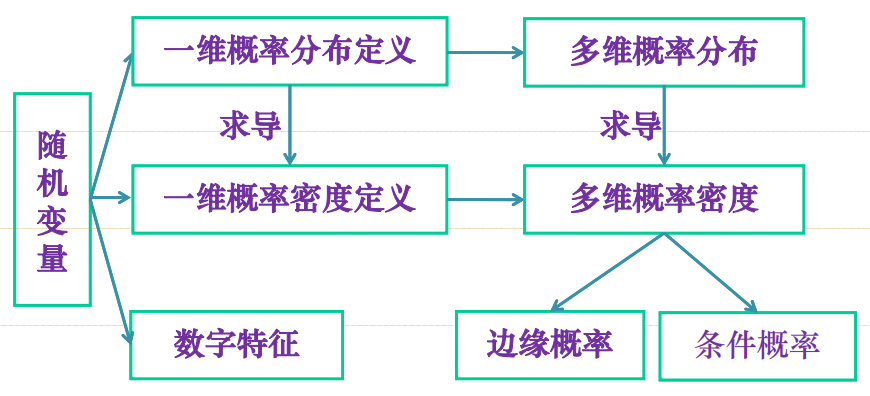
\includegraphics[scale=0.35]{1.png}
			\end{figure}
			\begin{figure}[H]
				\centering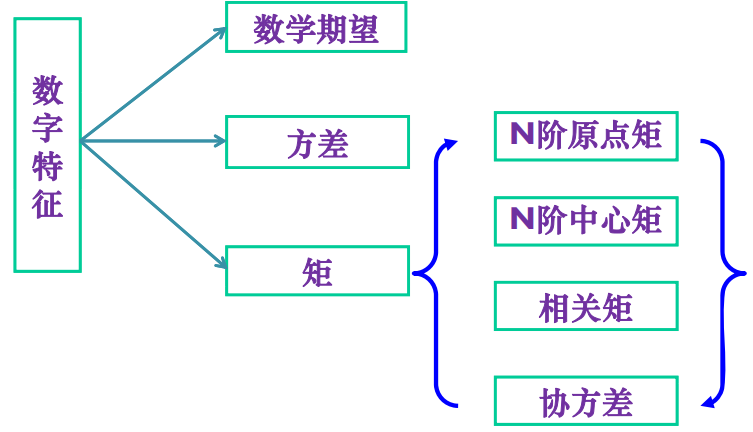
\includegraphics[scale=0.35]{2.png}
			\end{figure}
		
			\subsubsection{随机过程的数学定义}
			
				定义1:设E时随机试验,它的样本空间是$S=\{\xi\}$,对于每一个$\xi\subset \{S\}$,总有一个确定的时间函数$u(t,\xi)$与之对应。这样可得到一簇时间t的函数,该簇称为\uline{随机过程}。
				簇中的每一个函数称为这个随机过程的\uline{样本函数}。
			
				定义2:设E有一个过程$u(t)$,对于每一个时刻$t_j(j=1,2,...)$,$u(t_j)$时一个随机变量,则称$u(t)$为随机过程。(默认采用该定义描述)
				\begin{figure}[H]
					\centering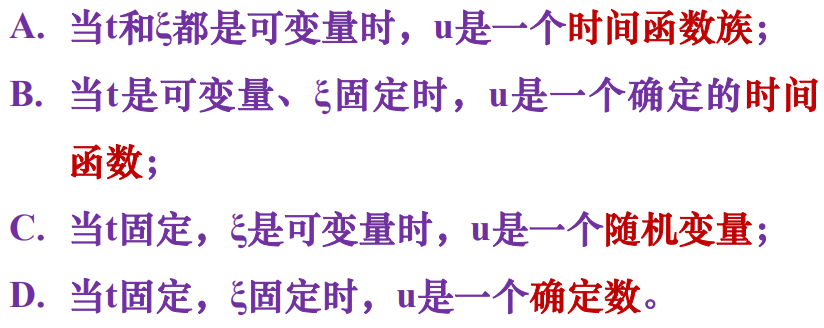
\includegraphics[scale=0.35]{3.png}
				\end{figure}
			
			\subsubsection{随机过程的分类}
				1.连续型随机过程:时间、状态都连续。
				\begin{figure}[H]
					\centering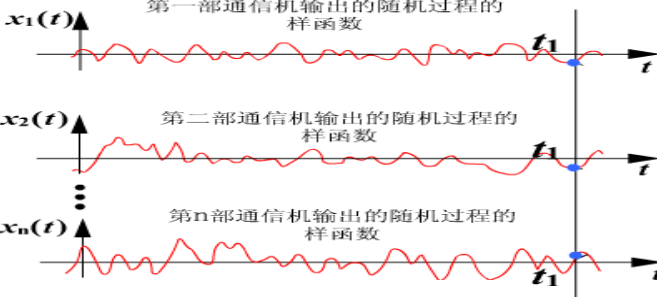
\includegraphics[scale=0.3]{4.png}
				\end{figure}
				2.离散时间型随机过程:时间离散,状态连续。
				\begin{figure}[H]
					\centering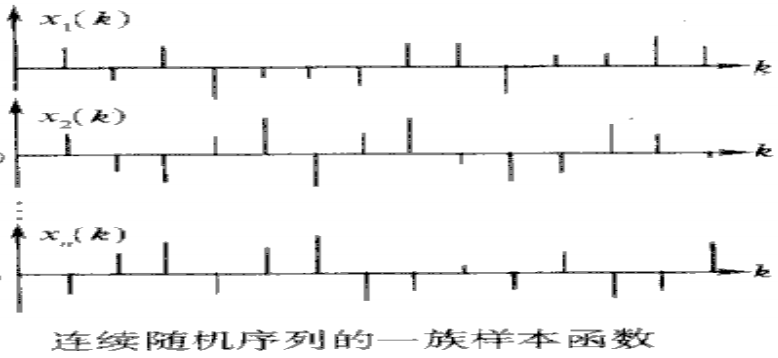
\includegraphics[scale=0.3]{5.png}
				\end{figure}
				3.离散幅度型随机过程:时间连续,状态离散。
				\begin{figure}[H]
					\centering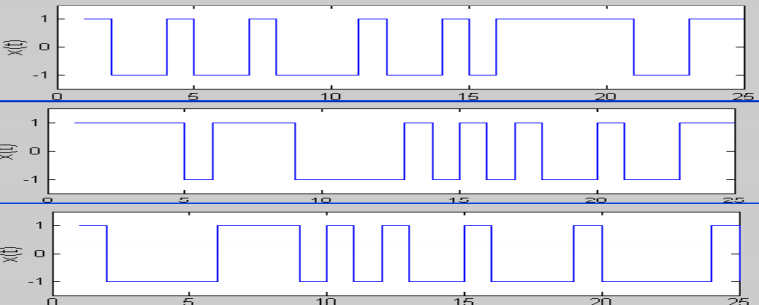
\includegraphics[scale=0.3]{6.png}
				\end{figure}
				4.离散型随机过程:时间、状态都离散。
				\begin{figure}[H]
					\centering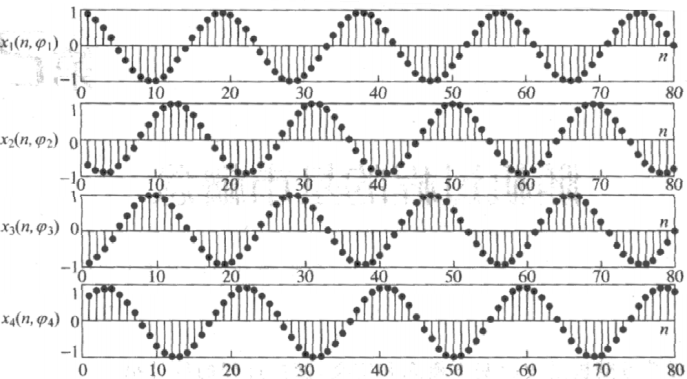
\includegraphics[scale=0.3]{7.png}
				\end{figure}
				(数字信号处理,处理的是第2种信号)
		\subsection{随机信号的时域(统计)表示}
			考虑由时间序列$u(n),u(n-1),\cdots,u(n-M+1)$示的离散时间随机过程$\{u(n)\}$。为了简化表示方式,从现在起,也使用$u(n)$表示该离散时间随机过程。(随机过程等价于\uline{多维随机变量})
			\subsubsection{随机信号的一维概率分布}
				对于一个随机过程$u(n)$,在任意时刻n是一个随机变量,它的\uline{一维概率分布函数}为:
				\[F_{u(n)}(u,n)= P\{u(n)\leq u\}\]
				若$F(u,n)$的一阶偏导数存在,则随机过程$u(n)$的\uline{一维概率密度函数}为:
				\[f_{u(n)}(u,n)=\frac{\partial F(u,n)}{\partial u}\]
			\subsubsection{随机信号的N维概率分布}	
				对于一个随机过程$u$,在任意N个时刻$n_1,n_2,\cdots,n_N$,可构成N维随机变量\\
				$\{u(n_1),u(n_2),\cdots ,u(n_N)\}$,它的的\uline{N维联合概率分布函数}为:
				\[F_u(u_1,u_2,\cdots,u_N;n_1,n_1,\cdots,n_N)= P\{u(n_1)\leq u_1,u(n_2)\leq u_2,\cdots, u(n_N)\leq u_N\}\]
				若$F_u(u_1,u_2,\cdots,u_N;n_1,n_1,\cdots,n_N)$对$u_1,u_2,\cdots, u_N$的偏导数存在,则随机过程$u(n)$的\uline{N维概率密度函数}为:
				\[f_u(u_1,u_2,\cdots,u_N;n_1,n_1,\cdots,n_N) = \frac{\partial^2F_u(u_1,u_2,\cdots,u_N;n_1,n_1,\cdots,n_N)}{\partial u_1\partial u_2\cdots\partial u_N}\]
				
			\subsubsection{离散时间随机过程的数字特征}		
				随机过程的数字特征有随机变量的数字特征推广而来,但一般不再是确定的数值,而是\uline{关于时间的函数}。
				
				\textbf{1.数学期望}:表示随机过程所有样本函数的统计平均函数。
				\[\mu(n)=E(u(n))=\int_{-\infty}^{+\infty}uf_{u(n)}(u,n)du\]
				
				\textbf{2.自相关函数}
				
				复数域:$r(n,n-k) = E[u(n)u^*(n-k)]$	
					
				实数域:$r(n,n-k) = E[u(n)u(n-k)]$
				\[k=0,\pm1,\pm2,...\]
				
				\textbf{3.自协方差函数}
				
				复数域:
				\[c(n,n-k) = E\{[u(n)-\mu(n)][u(n-k)-\mu(n-k)]^*\}\]	
				
				实数域:
				\[c(n,n-k) = E\{[u(n)-\mu(n)][u(n-k)-\mu(n-k)]\}\]				
				\[k=0,\pm1,\pm2,...\]
				
				分别减去了均值。
				
				\textbf{4.自相关函数与自协方差函数的关系}
				
				复数域:
				\[c(n,n-k) = r(n,n-k)-\mu(n)\mu^*(n-k)\]	
				
				实数域:
				\[c(n,n-k) =r(n,n-k)-\mu(n)\mu(n-k)\]				
				\[k=0,\pm1,\pm2,...\]
				
				当期望为0时,有$c(n,n-k) =r(n,n-k)$
				
				\textbf{5.广义平稳:}
				均值与时间无关,即$E(\mu(n))=\mu$,其自相关函数、自协方差函数与时间无关,只与样值之间的\uline{时间差}有关。
				即:$r(n,n-k)=r(k),\quad c(n,n-k)=c(k)$.
				
				\textbf{6.平均各态历经(遍历性):}
				对于广义平稳的随机过程,其均值和相关函数具有各态历经性,也称具有遍历性。
				具有具有\uline{各态历经性}的随机序列,可以用时间平均来获得集平均(期望)。
				
				随机过程的N个样本的时间平均为:
				\[\hat{\mu_N}=\frac{1}{N}\sum_{n=0}^{N-1}u(n)\]
				对于所有的N值,可得$E[\hat{\mu}_N]=\mu$,当$N\rightarrow \infty$时,有$\hat{\mu}_N=\mu$,则称随机过程在均值意义上是各态历经的,因为概率分布不随时间发生变化。
				
				\textbf{6.相关矩阵:}
				
				定义随机向量$\textbf{u}(n)=[u(n),u(n-1),\cdots,u(n-M+1)]^T$,则该随机过程的M为相关矩阵的定义为:
				
				复数域:$\textbf{R}=E[\textbf{u}(n)\textbf{u}^H(n)]$\quad(上标H表示转置及共轭操作)
				
				实数域:$\textbf{R}=E[\textbf{u}(n)\textbf{u}^T(n)]$
				
				\begin{figure}[H]
					\centering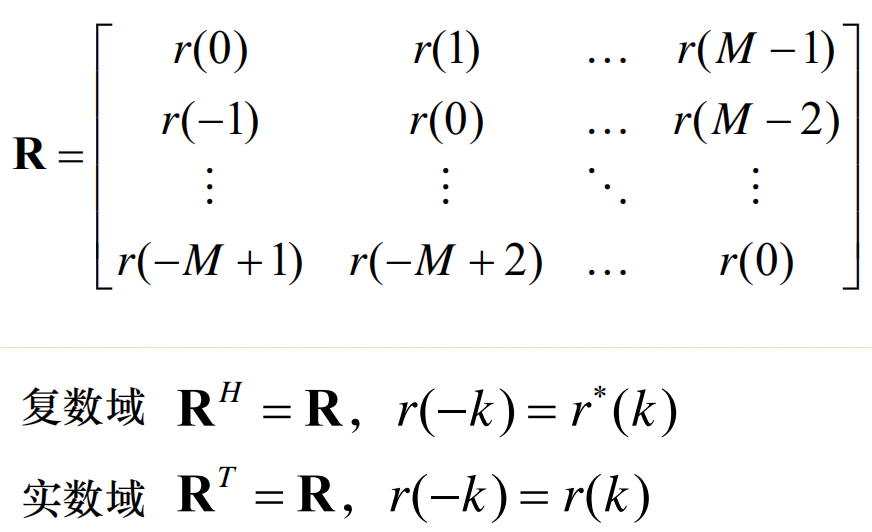
\includegraphics[scale=0.3]{8.png}
				\end{figure}
				
	\section{维纳滤波器}
		\begin{figure}[H]
			\centering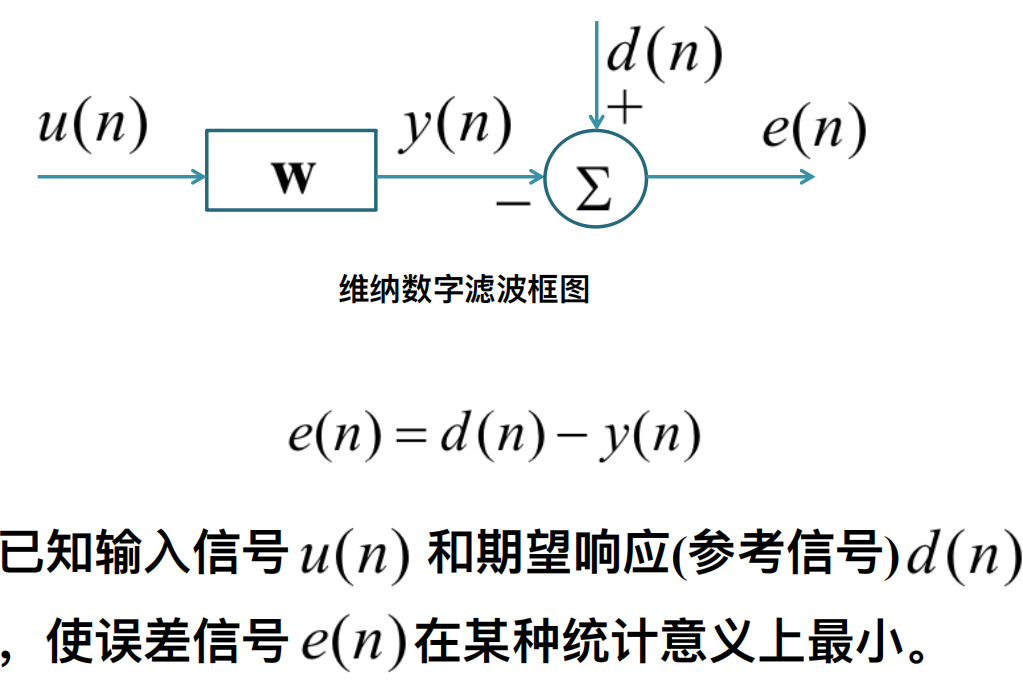
\includegraphics[scale=0.3]{9.png}
		\end{figure}
		\subsection{正交性原理}
		
			对于因果滤波器,其n时刻的输出为卷积:
			\[y(n) = \sum_{k=0}^\infty w_k^*u(n-k) = \textbf{w}^H\textbf{u}(n),\quad n=0,1,2\cdots\]
			使用均方误差作为代价函数,优点:该代价函数具有唯⼀的最⼩值。
			\[J(n) = E[|e(n)|^2]=E[e(n)e^*(n)]\] 
			
			如何求最小值:求函数对所有变量的偏导数,令所有偏导数为0,其对应的变量为多元函数取得最⼩值的解。为了⽅便表示,常将所有的偏导数写成列向量,该列向量称为函数的梯度或共轭梯度。因此,令所有偏导数为0,等价于令梯度或共轭梯度为0。
			
			第k个滤波器的系数可表示为:
			\[w_k = a_k=jb_k,\quad k=0,1,2,\cdots \]
			整个滤波器系数向量可表示为:
			\[\textbf{w} = \begin{bmatrix}
			w_0\\
			w_1\\
			\vdots\\
			w_{M-1}
			\vdots\\
			\end{bmatrix} =
			\begin{bmatrix}
			a_0+jb_0\\
			a_1+jb_1\\
			\vdots\\
			a_{M-1}+jb_{M-1}\\
			\vdots\\
			\end{bmatrix}\]\
			
			把代价函数$J(n)$对$\textbf{w}$中的每个$w_k$系数求偏导得到:
			\[\nabla_kJ = E\Bigg[\frac{\partial e(n)}{\partial a_k}e^*(n) +\frac{\partial e^*(n)}{\partial a_k}e(n)     + \frac{\partial e(n)}{\partial b_k}je^*(n) + \frac{\partial e^*(n)}{\partial b_k}je(n)\Bigg],\quad k=0,1,2,\cdots\]
			
			计算四个偏导数分别为:
			\begin{figure}[H]
				\centering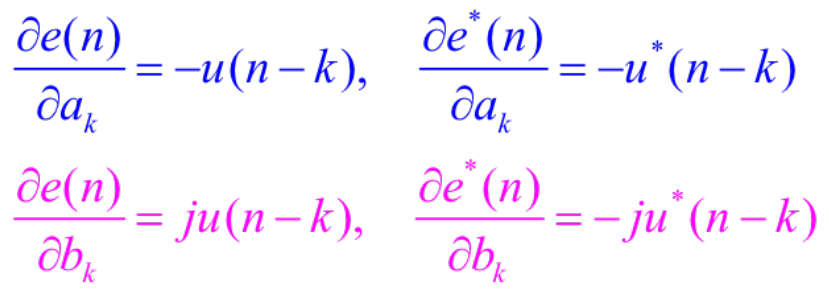
\includegraphics[scale=0.3]{10.png}
			\end{figure}
			
			将四个式子带入到$\nabla_kJ$,得到:
			\[\nabla_kJ = -2E[u(n-k)e^*(n)],\quad k=0,1,2,\cdots\]
			
			当梯度为零时,代价函数达到最小值,所以梯度向量$\nabla J$的所以元素都要等于0:
			\[\nabla_k J =-2E[u(n-k)e^*(n)] = 0 ,\quad k=0,1,2,\cdots\]
			
			等效于(下标o表示optimal):
			\[E[u(n-k)e_o^*(n)] = 0\]
			
			\textbf{正交性原理}:代价函数最小的充要条件是:估计误差$e_o(n)$与n时刻进入期望响应估计的每个输入样值$u(n-k)$正交。
			\begin{figure}[H]
				\centering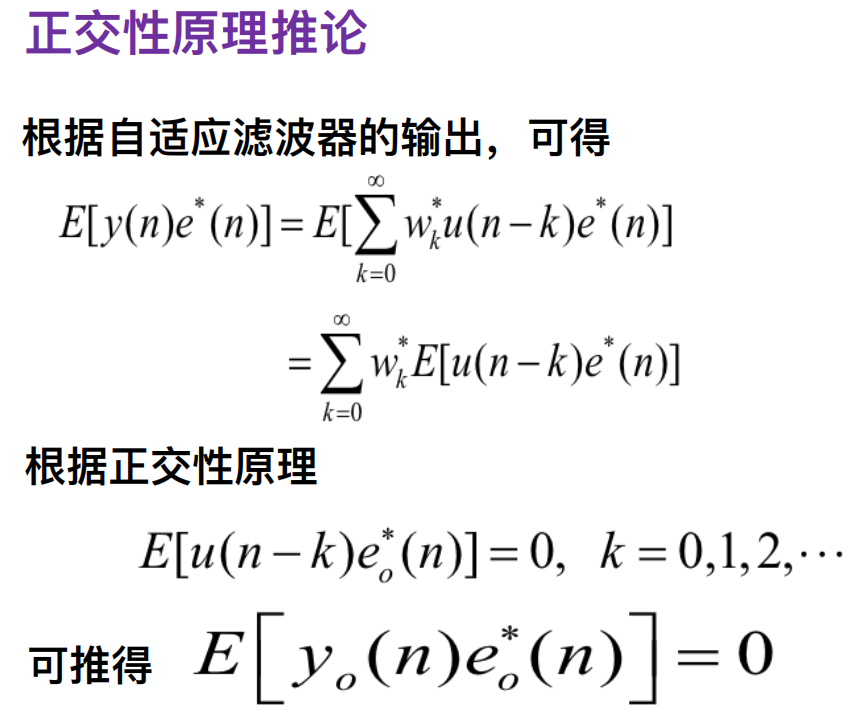
\includegraphics[scale=0.3]{11.png}
			\end{figure}
		\subsection{最小均方误差}
			达到最优时:
			\[e_o(n) = d(n) - y_o(n) = d(n) - \hat{d}(n|\mathcal{U}_n)\]
			$\mathcal{U}_n$表示输入限号$u(n)$直到时刻n的输入样值张成的空间。根据卷积公式,计算得到的输出实际上就是直到时刻n的输入样值的线性组合。
			\[d(n) = \hat{d}(n|\mathcal{U}_n) +e_o(n)\]	
			\[d^*(n) = \hat{d}^*(n|\mathcal{U}_n) +e_o^*(n)\]	
			
			所以:
			\[\sigma_d^2 = d(n)d^*(n) = \sigma_{\hat{d}(n|\mathcal{U}_n)}^2 + E[\hat{d}(n|\mathcal{U}_n)e_o^*(n)]+ E[\hat{d}^*(n|\mathcal{U}_n)e_o(n)]+ \sigma_{e_0}^2\]
			
			由正交性原理的推论可得,式子中的两项期望为0,所以有:
			\[\sigma_d^2 = \sigma_{\hat{d}}^2 + J_{min}\]
			\[ J_{min} = \sigma_d^2 - \sigma_{\hat{d}}^2\]
			
			归一化均方误差:
			\[\sigma = \frac{J_{min}}{\sigma_d^2} = 1-\frac{\sigma_{\hat{d}}^2}{\sigma_d^2}, \quad 0\leq \sigma\leq1\]
		\subsection{维纳-霍夫方程(求解)}	
			\begin{figure}[H]
				\centering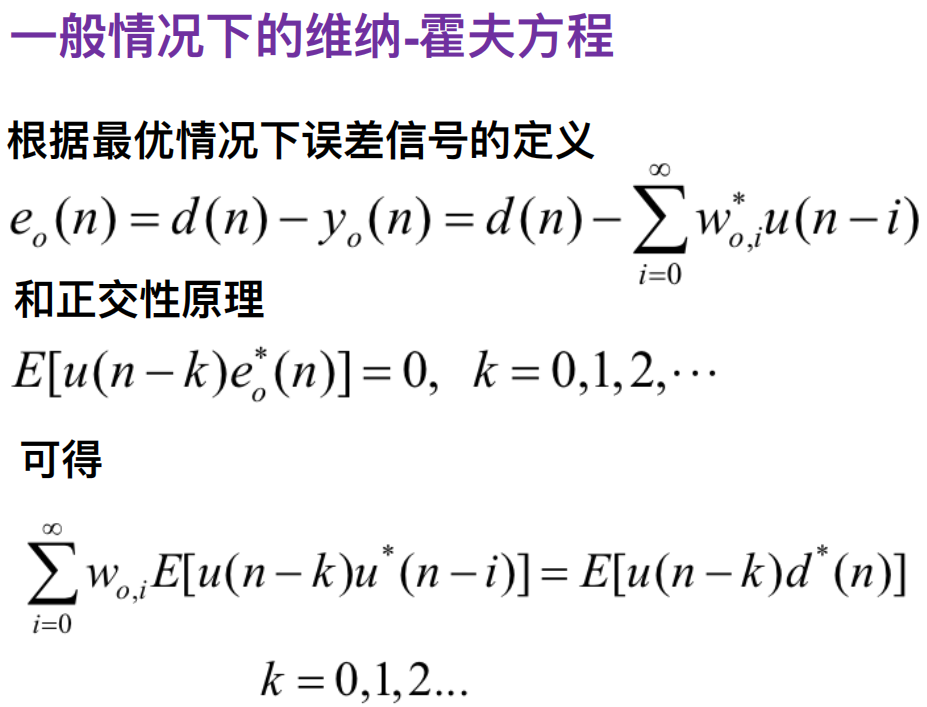
\includegraphics[scale=0.3]{12.png}
			\end{figure}
			\begin{figure}[H]
				\centering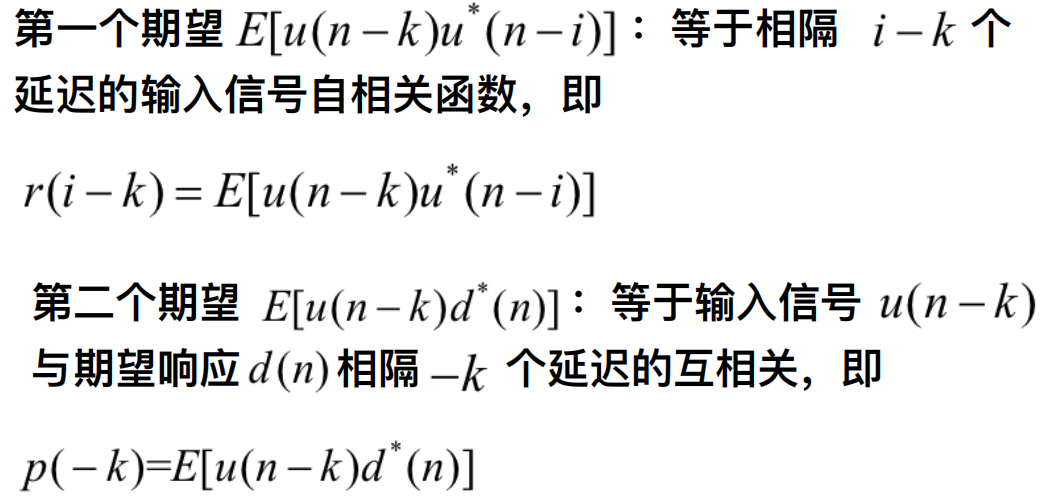
\includegraphics[scale=0.3]{13.png}
			\end{figure}
			
			将$r(i-k)$与$p(-k)$代入:

			\begin{figure}[H]
				\centering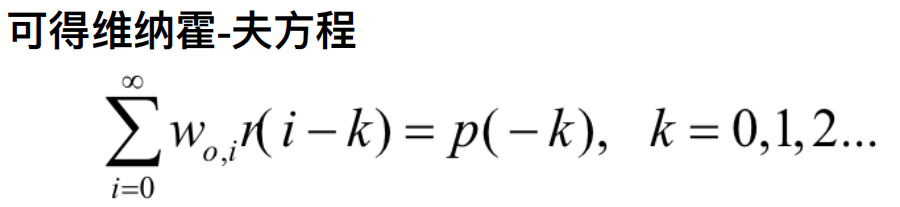
\includegraphics[scale=0.3]{15.png}
			\end{figure}
		
			\begin{figure}[H]
				\centering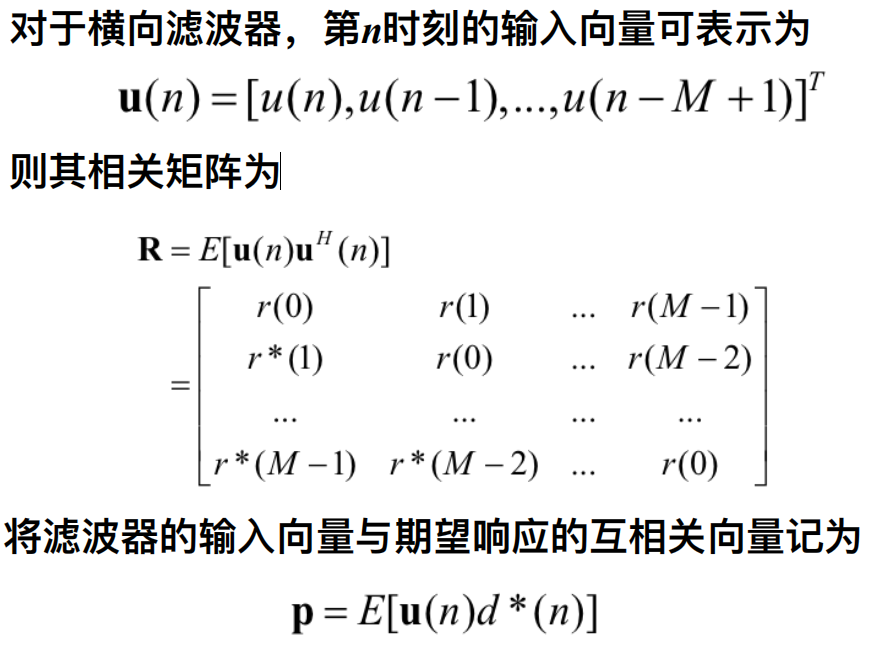
\includegraphics[scale=0.3]{16.png}
			\end{figure}
			\begin{figure}[H]
				\centering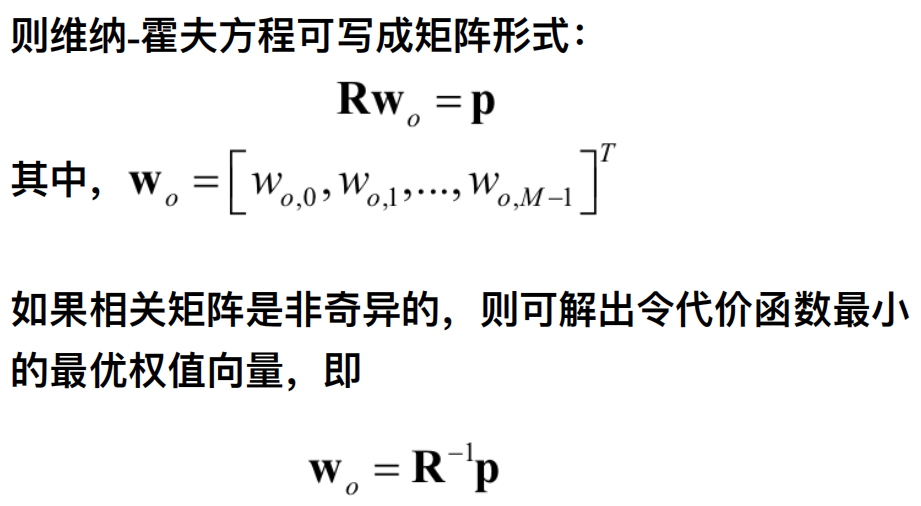
\includegraphics[scale=0.3]{17.png}
			\end{figure}
			
			\textbf{换个角度:利用向量求导来求解}
			
			误差:
			\[e(n) = d(n)-\textbf{w}^H\textbf{u}(n)\]
			
			误差的平方:
			\[\begin{aligned}
			e(n)e^*(n) &= \Big(d(n)-\textbf{w}^H\textbf{u}(n)\Big) \Big(d^*(n)-\textbf{u}^H(n)\textbf{w}\Big)\\
			&=|d(n)|^2 -d(n)\textbf{u}^H(n)\textbf{w}-\textbf{w}^H\textbf{u}(n)d^*(n) + \textbf{w}^H\textbf{u}(n)\textbf{u}^H(n)\textbf{w}
			\end{aligned}	
			\]
			
			对误差的平方取期望:
			\[\begin{aligned}
			E[|e(n)|^2] & =  E\big[|d(n)|^2\big] + E\big[d(n)\textbf{u}^H(n)\big]\textbf{w} + \textbf{w}^HE\big[\textbf{u}(n)d^*(n)\big] + \textbf{w}^HE\big[\textbf{u}(n)\textbf{u}^H(n)\big]\textbf{w}
			\end{aligned}
			\]
			其中$E\big[\textbf{u}(n)\textbf{u}^H(n)\big] = \textbf{R}$, 并令$E\big[\textbf{u}(n)d^*(n)\big] =\textbf{p} $(与维纳-霍夫方程中的记法相同),带入上式得损失函数:
			\[J(\textbf{w}) = E[|e(n)|^2]  = \sigma_d^2 - \textbf{p}^H\textbf{w} + \textbf{w}^H\textbf{p} +\textbf{w}^H\textbf{Rw}\]
			
			对上式求$\textbf{w}$的共轭梯度,并令其等于0:
			\[\frac{\partial J(\textbf{w})}{\partial\textbf{w}^*} = -\textbf{p} + \textbf{R} \textbf{w}=0\]
			同样可以求得参数$\textbf{w}$。
	\section{最速下降法}
		\subsection{最速下降法的基本思想}
			迭代下降法:从某一初始值$\textbf{w}(0)$开始,按照固定的步骤,产生一系列权重向量$\textbf{w}(1),\textbf{w}(2),\textbf{w}(3),\cdots $,使得代价函数的值在每一次迭代之后都下降:
			\[J(\textbf{w}(n+1)) < J(\textbf{w}(n))\]
			
			迭代下降法的一种简单形式——最速下降法,沿着负梯度方向连续调整权重向量$\textbf{w}$,
			将梯度表示为:
			\[\textbf{g} = \nabla J(\textbf{w})\]
			从而最速下降法可表示为($\mu$为步长):
			\[\textbf{w}(n+1) = \textbf{w}(n) -\frac{1}{2}\mu\textbf{g}(n)\]
		
		\subsection{最速下降算法应用于维纳滤波器}
			第2章中提到维纳滤波器的代价函数为:
			\[J(\textbf{w}) = E[|e(n)|^2]  = \sigma_d^2 - \textbf{p}^H\textbf{w}(n) + \textbf{w}^H(n)\textbf{p} +\textbf{w}^H(n)R\textbf{w}(n)\]
			其中:
			\[\begin{aligned}
			\sigma_d^2 &= E[d^2(n)]\\
			\textbf{p} &= E[\textbf{u}()d^*(n)]\\
			\textbf{R} &= E[\textbf{u}(n)\textbf{u}^H(n)]
			\end{aligned}\]
			其梯度向量为:
			\[\nabla J(n) = -2\textbf{p}+2\textbf{Rw}(n)\]
			代入最速下降法的公式中,迭代解为:
			\[\textbf{w}(n+1) = \textbf{w}(n) + \mu(\textbf{p}-\textbf{Rw}(n))\]
			
			【1】与维纳滤波器的闭合解$\textbf{w}_o=\textbf{R}^{-1}\textbf{p}$相比,迭代解不需要求相关矩阵$\textbf{R}$的逆。
			
			【2】迭代解是经典的最小均方算法的基础。
			
		\subsection{最速下降法的稳定性}	
			问:当$n\rightarrow\infty$时,是否有$\textbf{w}(n)\rightarrow\textbf{w}_o$?若有,需要满足什么条件?
			
			\uline{定义}:n时刻的权重误差向量:
			\[\textbf{c}(n) = \textbf{w}_o -\textbf{w}(n)\]
			将迭代式:
			\[\textbf{w}(n+1) = \textbf{w}(n) + \mu(\textbf{p}-\textbf{Rw}(n))\]
			两边同时减去$\textbf{w}_o$,并消去负号,可得:
			\[\textbf{c}(n+1) = \textbf{c}(n) - \mu(\textbf{p}-\textbf{Rw}(n))\]
			将维纳方程$\textbf{Rw}_o=\textbf{p}$代入上式,消去$\textbf{p}$,可得:
			\[\textbf{c}(n+1) = \textbf{c}(n) -\mu\textbf{R}(\textbf{w}_o-\textbf{w}(n))\]
			\[\textbf{c}(n+1) = (\textbf{I}-\mu\textbf{R})\textbf{c}(n)\]
			根据上式的误差向量的关系类推,得到:
			\[\textbf{c}(n+1) = (\textbf{I}-\mu\textbf{R})^2\textbf{c}(n-1)\]
			\[\textbf{c}(n+1) = (\textbf{I}-\mu\textbf{R})^{n+1}\textbf{c}(0)\]
			每一次迭代之后误差向量都乘上了$(\textbf{I}-\mu\textbf{R})$,如果该项小于0,那么误差向量是在不断减小的。
			
			\uline{使用特征值分解},将相关矩阵分解为:
			\[\textbf{R} = \textbf{Q}\Lambda\textbf{Q}^H\]
			迭代式变为:
			\[\textbf{c}(n+1) = (\textbf{I}-\mu\textbf{Q}\Lambda\textbf{Q}^H)\textbf{c}(n)\]
			两边同乘以$\textbf{Q}^H$:
			\[\begin{aligned}
			\textbf{Q}^H\textbf{c}(n+1) &= (\textbf{Q}^H-\mu\Lambda\textbf{Q}^H)\textbf{c}(n)\\
			&=(\textbf{I}-\mu\Lambda)\textbf{Q}^H\textbf{c}(n)
			\end{aligned}\]
			定义变换向量$\textbf{v}(n)=\textbf{Q}^H\textbf{c}(n)$,代换后有:
			\[\textbf{v}(n+1) = (\textbf{I}-\mu\Lambda)\textbf{v}(n)\]
			初始权重常取$\textbf{w}(0) = \textbf{0}$,所以:
			\[\textbf{v}(0) = \textbf{Q}^H\textbf{c}(0) = \textbf{Q}^H[\textbf{w}_o-\textbf{0}] = \textbf{Q}^H\textbf{w}_o\]
			\begin{figure}[H]
				\centering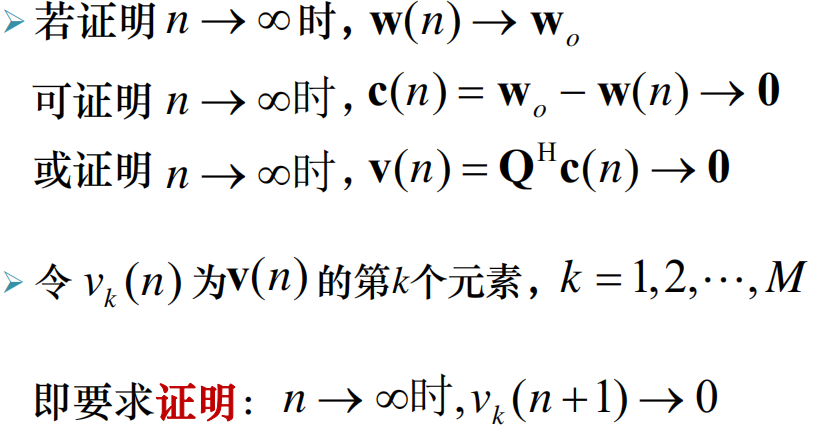
\includegraphics[scale=0.3]{18.png}
			\end{figure}
			\begin{figure}[H]
				\centering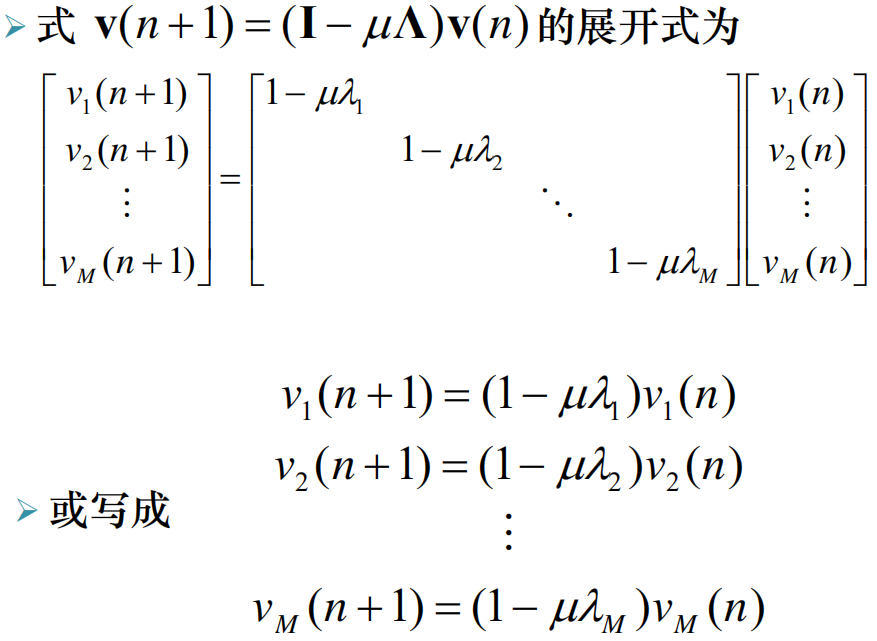
\includegraphics[scale=0.3]{19.png}
			\end{figure}
			\begin{figure}[H]
				\centering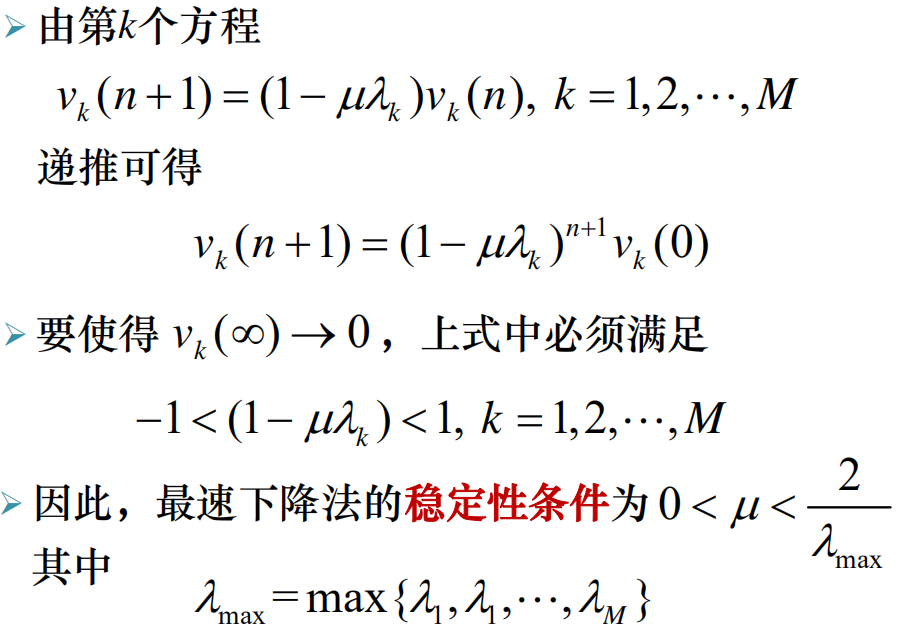
\includegraphics[scale=0.3]{20.png}
			\end{figure}
			
			
			
			
	\section{自适应滤波器}
		

\end{document}